\chapter{State of the Art}
\label{chap:state_of_the_art}

The state of the art is the information relevant to the study that will be done. In this way, we can close 
the scope of what this new investigation will prove and find studies that can help us close that new research 
gap. As a small reminder, display polarity is the mode that will be shown on the screen, positive polarity 
being dark characters in bright background and negative polarity the other way around.

\section{Previous Studies}
The previous studies section, as explained above, consists of doing research in order to slowly close the 
research gap. This process was done by following a “baking” process, where an initial research was done on 
the subject in several Databases such as IEEExplore\cite{ieee_explore} or Scopus\cite{scopus}, refining the keywords every time to 
find related articles. The best keywords appeared to be:
\begin{itemize}
    \item Display polarity
    \item Visual fatigue
    \item Reading
\end{itemize}
After reading and analyzing the first bake, a second bake of refinement and vertical expansion (analyzing cites and 
references of such scientific papers) was done. After erasing the unrelated articles and the ones out of scope, 
the following key articles were found:


\subsection{The impact of web page text-background colour combinations on readability, retention, aesthetics and behavioural intention\cite{Hall2004}}
\begin{table}[H]   
    \centering
    \caption{Summary of the article by Hall and Hanna}
    \label{tab:hall2004}
    \begin{tabular}{|p{0.18\textwidth}|p{0.72\textwidth}|}
        \hline
        \textbf{Authors} & Hall, Richard H \\
                         & Hanna, Patrick \\ \hline
        \textbf{Year}    & 2004 \\ \hline
        \textbf{Source}  & Behaviour and Information Technology \\ \hline
        \textbf{DOI}     & \url{10.1080/01449290410001669932} \\ \hline
    \end{tabular}
\end{table}

\subsubsection{Reason for choice} 
The motivation to use this paper as a reference is because of the Likert scale questionnaire that is used, giving questions 
that can perfectly fit with the desired study. In addition, they hand out more questions that could be applied to further 
explain other non-studied parts of my thesis. 

\subsection{Study on the effects of display color mode and luminance contrast on visual fatigue. \cite{Xie2021}}
\begin{table}[H]   
    \centering
    \caption{Summary of the article by Xie \textit{et al.}}
    \label{tab:xie2021}
    \begin{tabular}{|p{0.18\textwidth}|p{0.72\textwidth}|}
        \hline
        \textbf{Authors} & Xie, Xiaojiao \\
                         & Song, Fanghao \\
                         & Liu, Yan \\
                         & Wang, Shurui \\
                         & Yu, Dong \\ \hline
        \textbf{Year}    & 2021 \\ \hline
        \textbf{Source}  & IEE Access \\ \hline
        \textbf{DOI}     & \url{10.1109/ACCESS.2021.3061770} \\ \hline
    \end{tabular}
\end{table}

\subsubsection{Reason for choice}
This study is one of the closest to what the purpose of this thesis is related to. However,
 there are some differences. For example, the aim is different, and they are not focused on 
 usability. Nevertheless, this paper has provided good information to reach the desired 
 experiment for investigating the usability and visual fatigue. In the following illustration 
 we can see the luminance contrast: (a) 0.969, (b) 0.935, (c) 0.855, (d) 0.868, (e) 0.725, (f) 0.469
\begin{figure}[H]
    \centering
    % Primer grupo (Izquierdo: a,b,c)
    \begin{subfigure}[b]{0.48\textwidth}
        \centering
        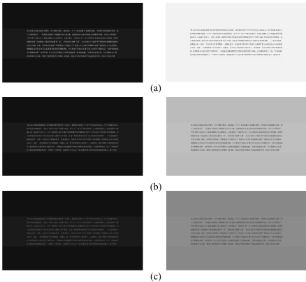
\includegraphics[width=\textwidth]{figures/luminance_contrast_1.png}
    \end{subfigure}
    \hfill % Separador d las dos imagenes
    % Segundo grupo (Derecho: d,e,f)
    \begin{subfigure}[b]{0.48\textwidth}
        \centering
        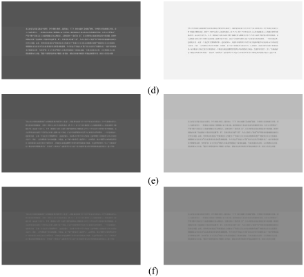
\includegraphics[width=\textwidth]{figures/luminance_contrast_2.png}
    \end{subfigure}
    
    \caption{Experimental Illustrations.}
    \label{fig:experimental_illustrations_all}
\end{figure}
\begin{figure}[H]
    \centering
    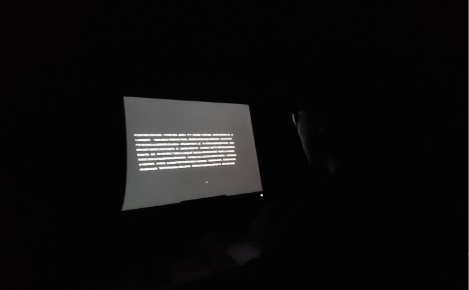
\includegraphics[width=0.8\textwidth]{figures/luminance_participation.png}
    \caption{Photo of participant during the experiment}
    \label{fig:luminance_participation}
\end{figure}


\subsection{The Effect of Display Polarity on Reading Speed and Reading Error Among Young Adults.\cite{Muhamad2024}}
\begin{table}[ht]   
    \centering
    \caption{Summary of the article by Muhamad and Mokhtar}
    \label{tab:muhamad2024}
    \begin{tabular}{|p{0.18\textwidth}|p{0.72\textwidth}|}
        \hline
        \textbf{Authors} & Muhamad, Nurulain \\
                         & Mokhtar, Nurliyana \\ \hline
        \textbf{Year}    & 2024 \\ \hline
        \textbf{Source}  & Journal of Health Science and Medical Research \\ \hline
        \textbf{DOI}     & \url{10.31584/jhsmr.20241095} \\ \hline
    \end{tabular}
\end{table}
\subsubsection{Reason for choice}
The reason for choosing this article is the fact that, even though the study is quite similar, they 
are not using an eye tracker but instead measuring times by hand, hence giving a general measurement 
with a lot of imprecisions. However, the methodology (without considering the tools for measuring) is 
an acceptable one, and some of it is considered while processing the data.

\begin{figure} [H]
    \centering
    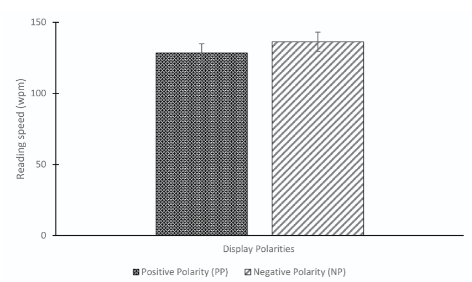
\includegraphics[width=0.8\textwidth]{figures/reading_speed_Muhamad.png}
    \caption{The comparison of reading speed between positive and negative display polarities.}
    \label{fig:reading_speed}
\end{figure}
Results:  
Reading speed, measured in words per minute (wpm), differed significantly between polarities, with negative 
polarity yielding higher speeds (136.27±25.58 wpm) compared to positive polarity (128.42±19.98 wpm), 
Z=-2.355, p-value\&lt;0.05. However, no significant polarity-related differences were found in reading errors, 
including mispronunciation (p-value=0.193) or omission (p-value=0.113).   Conclusion: Negative polarity 
displays enhanced reading performance by increasing reading speed; while reading errors remained unaffected.

